\documentclass[12pt,a4paper]{article}
\usepackage[utf8]{inputenc}
\usepackage[russian]{babel}
\usepackage[OT1]{fontenc}
\usepackage{mathtools}
\usepackage{amsfonts}
\usepackage{amssymb}
\usepackage{enumitem}
\usepackage{alltt}
\usepackage{graphicx}
\usepackage{indentfirst}
\usepackage{caption}
\usepackage{float}
\usepackage{wrapfig}
\usepackage{physics}
\usepackage{multirow}
\usepackage{longtable}
\usepackage{amsmath,amsfonts,amssymb,amsthm,mathtools}
\usepackage{icomma}
\setlength{\parindent}{0.75cm}
\graphicspath{{pictures/}}
\DeclareGraphicsExtensions{.png}
\usepackage[left=15mm,right=15mm,top=2cm,bottom=2cm]{geometry}
\author{Глотов Алексей}
\begin{document}
\newpage
\begin{center}
\footnotesize{{ГОСУДАРСТВЕННОЕ АВТОНОМНОЕ ОБРАЗОВАТЕЛЬНОЕ УЧРЕЖДЕНИЕ}\break
{ВЫСШЕГО ОБРАЗОВАНИЯ}
\break
{\bf {МОСКОВСКИЙ ФИЗИКО-ТЕХНИЧЕСКИЙ ИНСТИТУТ}}
\break
\small{(НАЦИОНАЛЬНЫЙ ИССЛЕДОВАТЕЛЬСКИЙ УНИВЕРСИТЕТ)}}
\break
\hfill \break
\hfill \break
\begin{center}
\normalsize{Кафедра общей физики}
\end{center}
\hfill \break
\hfill \break
\hfill \break
\hfill \break

\begin{center}
\normalsize {Лабораторная работа 2.3.1}
\end{center}
\hfill \break\\
\large{\textbf{Получение и измерение вакуума}}
\end{center}
\begin{flushleft}
\hfill \break
\hfill \break
\hfill \break
\hfill \break
\hfill \break
\hfill \break
\hfill \break
\hfill \break
\hfill \break
\hfill \break
\hangindent=9cm
\normalsize{Преподаватель:}\hfill
\normalsize{доцент Игуманов А.Ю.}\\
\hfill \break
\normalsize{Обучающийся:}\hfill
\normalsize{Глотов А.А} \\
\hfill \break
\end{flushleft}
\hfill \break
\hfill \break
\hfill \break
\hfill \break
\hfill \break
\hfill \break
\hfill \break
\hfill \break
\hfill \break
\hfill \break
\hfill \break

\begin{center}
Долгопрудный \break
 2022
\end{center}

\thispagestyle{empty}


\newpage
\section{Введение}

\subsection{Аннотация}

Данная работа посвящена изучению явления установления вакуума в системе. Используются следующие методы: линеаризация и анализ графиков зависимости p(t). Значения времени t получаем с помощью секундомера, давления p - с помощью электронных манометров

\textbf{Цель работы:} 1) измерение объёмов форвакуумной и высоковакуумной частей установки; 2) определение скорости откачки системы в стационарном режиме, а также по ухудшению и по улучшению вакуума.

\textbf{В работе используются:} вакуумная установка с манометрами: масляным, термопарным и ионизационным.

\subsection{Теоретические сведения}

По степени разряжения вакуумные установки принято делить на три класса: 1) низковакуумные -- до $10^{-2}$-$10^{-3}$ торр; 2) высоковакуумные -- $10^{-4}$-$10^{-7}$ торр; 3) установки сверхвысокого вакуума -- $10^{-8}$-$10^{-11}$ торр. С физической точки зрения низкий вакуум переходит в высокий, когда длина свободного пробега молекул газа оказывается сравнима с размерами установки; сверхвысокий вакуум характерен крайней важностью процессов адсорбции частиц на поверхности вакуумной камеры.

\subsection*{Процесс откачки}

Обозначим через $Q_d$ количество газа, десорбирующегося с поверхности откачиваемого объема в единицу времени, через $Q_i$ — количество газа, проникающего в единицу времени в этот объем извне — через течи. Будем считать, что насос обладает скоростью откачки $W$ и в то же время сам является источником газа; пусть $Q_n$ — поток газа, поступающего из насоса назад в откачиваемую систему. Будем измерять количество газа $Q_d$, $Q_i$ и $Q_n$ в единицах $PV$ (легко видеть, что это произведение с точностью до множителя $RT/ \mu$ равно массе газа). Основное уравнение, описывающее процесс откачки, имеет вид

\begin{equation}
\label{otkachka}
	-VdP=(PW-Q_d-Q_n-Q_i)dt.
\end{equation}

Левая часть этого уравнения равна убыли газа в откачиваемом объеме $V$ , а правая определяет количество газа, уносимого насосом, и количество прибывающего вследствие перечисленных выше причин
за время $dt$. При достижении предельного вакуума (давление $P_{pr}$)

\begin{equation}
\label{predel_1}
	\frac{dP}{dt}=0,
\end{equation}

\begin{equation}
\label{predel_2}
	W=\frac{\sum Q_i}{P_{pr}}.
\end{equation}

Обычно $Q_i$ постоянно, a $Q_n$ и $Q_d$ слабо зависят от времени, поэтому в наших условиях все эти члены можно считать постоянными. Считая также постоянной скорость откачки $W$ , уравнение~(\ref{otkachka}) можно проинтегрировать и, используя~(\ref{predel_1}), получить
\begin{equation}
\label{davlenie}
	P = P_o \exp{(-\frac{W}{V} t)} + P_{pr}.
\end{equation}

\subsection*{Течение газа через трубу}

Для количества газa, протекающего через трубу в условиях высокого вакуума или, как говорят, в кнудсеновском режиме, справедлива формула

\begin{equation}
\label{formula}
	\frac{d(PV)}{dt}=\frac{4}{3}r^3 \sqrt{\frac{2\pi RT}{\mu}} \frac{P_2-P_1}{L}.
\end{equation}
Применим эту формулу к случаю, когда труба соединяет установку с насосом.
Пренебрежем давлением $P_1$ у конца, обращенного к насосу. Будем измерять количество газа, покидающего установку при давлении $P = P_2$. Пропускная способность трубы

\begin{equation}
	C_{tr}=(\frac{dV}{dt})_{tr}=\frac{4}{3}\frac{r^3}{L}\sqrt{\frac{2\pi RT}{\mu}}.
\end{equation}

	Мы видим, что пропускная способность зависит от радиуса трубы в третьей степени и обратно пропорциональна ее длине. В вакуумных установках следует поэтому применять широкие короткие  трубы.
	
	При расчете вакуумных систем нужно принимать во внимание также пропускную способность отверстий, например, в кранах. Для диффузионного насоса можно считать, что каждая молекула воздуха, попавшая в кольцевой зазор между соплом и стенками насоса, увлекается струей пара и не возвращается обратно в откачиваемый объем. Скорость откачки такого насоса можно считать равной пропускной способности отверстия с площадью, равной площади кольцевого зазора, т. е. насос качает как кольцевой зазор, с одной стороны которого расположен откачиваемый объем, а с другой -- пустота.


\subsection{Схема эксперимента}

\subsection*{Процесс откачки}
	Производительность насоса определяется скоростью откачки $W$ (л/с): $W$ — это объем газа, удаляемого из сосуда при данном давлении за единицу времени. Скорость откачки форвакуумного насоса равна емкости воздухозаборной камеры, умноженной на число оборотов в секунду.
Рассмотрим обычную схему откачки. Разделим вакуумную систему на две части: «откачиваемый объем» (в состав которого включим используемые для работы части установки) и «насос», к которому, кроме самого насоса, отнесем трубопроводы и краны, через которые производится откачка нашего объема. 

	Отметим, что для проведения экспериментов необходимо нагреть нашу систему до рабочей температуры. Индикатором нагрева служит масло, начинающее капать при определенных температурах и давлении, увеличивая интенсивность со временем.

\subsection*{Течение газа через трубу}
	Характер течения газа существенно зависит от соотношения между размерами системы и длиной свободного пробега молекул. При атмосферном давлении и даже при понижении давления до форвакуумного длина свободного пробега меньше диаметра трубок и течение откачиваемого газа определяется его вязкостью, т. е. взаимодействием его молекул. При переходе к высокому вакууму картина меняется. Столкновения молекул между собой начинают играть меньшую роль, чем соударения со стенками. Течение газа в трубе напоминает в этих условиях диффузию газа из области больших концентраций в области, где концентрация ниже, причем роль длины свободного пробега играет ширина трубы.
	
	
\subsection{Методика измерений}

\begin{enumerate}
\item
	Определим объемы форвакуумной и высоковакуумной частей установки. Сначала впустим атмосферу в установку. Запрем воздух при комнатных условиях в капилляре между кранами 5 и 6. После этого откачаем воздух из оставшейся части установки (сделав это в два этапа - сначала насос должен откачать сам себя, а только потом - установку). После этого мы сначала высвободим запертый воздух только в ФВ часть, а затем добавим к ней и ВВ. Тогда записав уравнение Менделеева-Клапейрона и зная объем капилляра, мы найдем объемы соответствующих частей установки:
\begin{equation}
	P_0 V_0 = P_{\text{уст}} (V_{\text{фв}} + V_{\text{вв}}),
\end{equation}
где $P_0$ -- атмосферное давление; $V_0$ -- объем капилляра и кранов 5 и 6; $P_{\text{уст}}$ -- установившееся давление; $V_{\text{фв}}$ и $V_{\text{вв}}$ -- соответственно объемы форвакуумной и высоковакуумной частей.
	
\item
	Для измерения скорости откачки диффузионного насоса измерим улучшение вакуума во времени. Построим график зависимости $-\ln{\frac{P-P_{\text{пр}}}{P_0}}$ от $t$. Из формулы~(\ref{davlenie}) следует, что наклон, построенной кривой, есть $W / V$

\item
	Откроем кран 6 и создадим исскуственную течь через капилляр. Рассчитаем производительность насоса по различию $P_{\text{gh}}$ и $P_u$, где $P_u$ -- установившееся давление в высоковакуумной части с искусственной течью. В условиях высокого вакуума справдлива формула~(\ref{formula}), где положим $P_1 := P_u$, $P_2$ -- давление в форвакуумной части. 

\subsection{Экспериментальная установка}

Установка изготовлена из стекла,
 и состоит из форвакуумного баллона (ФБ), высоковакуумного диффузионного насоса (ВН), высоковакуумного баллона (ВБ), масляного (М) и ионизационного (И) манометров, термопарных манометров ($\text{М}_1$ и $\text{М}_2$), форвакуумного насоса (ФН) и соединительных кранов ($К_1, К_2,..., К_6$) (Рис. 1). Кроме того, в состав установки входят: вариатор (автотрансформатор с регулируемым выходным напряжением), или реостат и амперметр для регулирования тока нагревателя диффузионного насоса. \\
  \begin{figure}[h]
 	\centering
 	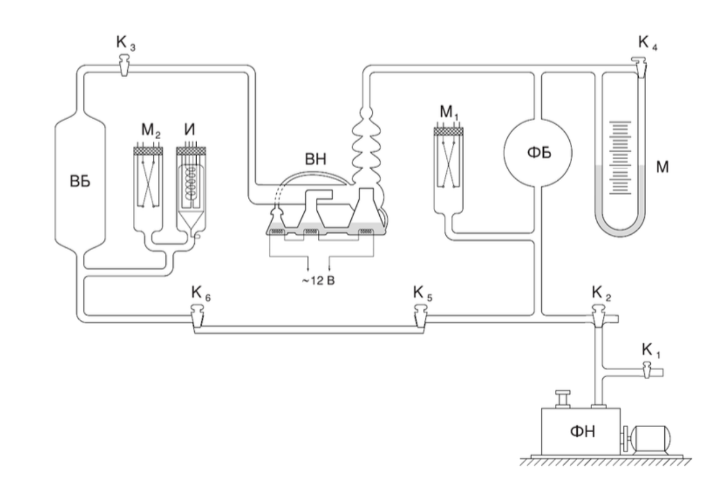
\includegraphics[width=0.5 \textheight]{2.3.1_1}
 	\caption{Схема установки}
 	\label{fig:Схема установки}
 \end{figure}

\begin{figure}[t]
	\centering
	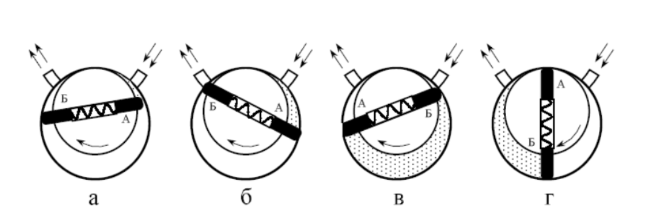
\includegraphics[width=0.7\linewidth]{2.3.1_2}
	\caption[]{Схема действия ротационного двухпластинчатого форвакуумного насоса}
	\label{fig:Схема ФВ насоса}
\end{figure}

Кран $К_1$ используется для заполнения форвакуумного насоса и вакуумной установки атмосферным воздухом. Во время работы установки
он должен быть закрыт. Трёхходовой кран $К_2$ служит для соединения
форвакуумного насоса с установкой или атмосферой. Кран $К_3$ отделяет
высоковакуумную часть установки от форвакуумной. Кран $К_4$ соединяет между собой колена масляного манометра. Он должен быть открыт во все время работы установки и закрывается лишь при измерении
давления в форвакуумной части. Краны $К_5$ и $К_6$ стоят по концам капилляра и соединяют его с форвакуумной и высоковакуумной частями установки. 


Устройство одной ступени масляного диффузионного насоса схематически показано на Рис. 3 (в лабораторной установке используется несколько откачивающих ступеней). Масло, налитое в сосуд, подогревается электрической печкой. Пары масла поднимаются по трубе и вырываются из сопла. Струя паров увлекает молекулы газа, которые поступают из откачиваемого сосуда через трубку. Дальше смесь попадает в вертикальную трубу. Здесь масло осаждается на стенках трубы и маслосборников и стекает вниз, а оставшийся газ откачивается форвакуумным насосом. 


\begin{figure}[H]
\centering
	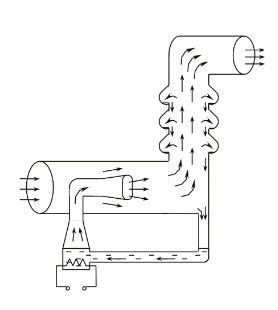
\includegraphics{2.3.1_3} 
	\caption{Схема работы одной ступени диффузионного насоса} 
\end{figure}

\newpage
\section{Результаты измерений и обработка данных}

\subsection{Определение характеристик установки}

Запишем характеристики нашей экспериментальной установки: \hfill \break
$$\rho_{\text{масло}} = 0.885\frac{\text{г}}{\text{см}^3}$$
$$V_{\text{атм}} = 50 \text{см}^3$$
$$p_{\text{атм}} = 102,6\text{кПа}$$
$$L = 10 \text{см} \;\;\;\;\;\;\; d = 0.8 \text{мм}$$
Установим значения объемов, используемых в нашей работе.

$h_{1} = (346 \pm 1)\text{мм} \;\;\;\;\;\; h_{2} = (50 \pm 1)\text{мм}$ \hfill \break
$h_{3} = (298 \pm 1)\text{мм} \;\;\;\;\;\; h_{4} = (111 \pm 1)\text{мм}$

Согласно закону Бойля-Мариотта, получим следующие уравнения:

\begin{equation}
V_{\text{фв}} = V_{0}\frac{p_{0}}{\Delta{p}_{1}} = V_{0}\frac{p_{0}}{\rho{g}(h_{1}-h_{2})} = (2005 \pm 46)\text{см}^3
\end{equation}

\begin{equation}
V_{\text{вв}} = V_{0}\frac{p_{0}}{\Delta{p}_{2}} - V_{\text{фв}} = \frac{V_{0}p_{0}}{\rho{g}}(\frac{1}{h_{3}-h_{4}}-\frac{1}{h_{1}-h_{2}}) = (1165 \pm 41)\text{см}^3
\end{equation}

\subsection{Получение вакуума}

Проведем настройку установки для следующей серии измерений

$p_{\text{пр}} = 6,5*10^{-5}$мм.рт.ст 

Снимем зависимость p(t) и запишем полученные данные в таблицу

\begin{center}
\begin{tabular}{|c|c|c|c|c|c|c|c|}
\hline 
p, мм.рт.ст.$*10^{-5}$ & t,c  & p, мм.рт.ст.$*10^{-5}$ & t,c  & p, мм.рт.ст.$*10^{-5}$ & t,c  & p, мм.рт.ст.$*10^{-5}$ & t,c  \\ 
\hline 
72 & 0 & 33 & 6 & 13 & 12 & 8.6 & 21 \\ 
\hline 
71 & 1 & 30 & 6 & 12 & 13 & 8.5 & 21 \\ 
\hline 
70 & 1 & 27 & 7 & 11 & 14 & 8.4 & 22 \\ 
\hline 
68 & 1 & 25 & 8 & 10 & 16 & 8.3 & 22 \\ 
\hline 
66 & 2 & 23 & 8 & 9.8 & 17 & 8.2 & 23 \\ 
\hline 
61 & 2 & 21 & 8 & 9.6 & 18 & 8.1 & 25 \\ 
\hline 
58 & 3 & 19 & 9 & 9.4 & 18 & 8.0 & 26 \\ 
\hline 
54 & 4 & 18 & 9 & 9.3 & 18 & 7.9 & 29 \\ 
\hline 
48 & 4 & 17 & 10 & 9.1 & 19 & 7.8 & 32 \\ 
\hline 
45 & 4 & 16 & 10 & 9.0 & 19 & 7.7 & 37 \\ 
\hline 
40 & 5 & 15 & 11 & 8.8 & 20 & 7.6 & 53 \\ 
\hline 
36 & 6 & 14 & 11 & 8.7 & 20 & - & - \\ 
\hline 
\end{tabular} 
Улучшение вакуума
\end{center}

\begin{center}
\begin{tabular}{|c|c|c|c|c|c|c|c|}
\hline 
p, мм.рт.ст$*10^{-5}$ & t,c & p, мм.рт.ст$*10^{-5}$ & t,c & p, мм.рт.ст$*10^{-5}$ & t,c & p, мм.рт.ст$*10^{-5}$ & t,c \\ 
\hline 
7.6 & 0 & 21 & 14 & 40 & 35 & 59 & 57 \\ 
\hline 
7.7 & 1 & 22 & 15 & 41 & 36 & 60 & 59 \\ 
\hline 
7.8 & 1 & 23 & 16 & 42 & 37 & 61 & 60 \\ 
\hline 
8.0 & 1 & 24 & 17 & 43 & 38 & 62 & 61 \\ 
\hline 
8.3 & 2 & 25 & 18 & 44 & 39 & 63 & 63 \\ 
\hline 
8.7 & 2 & 26 & 19 & 45 & 40 & 64 & 63 \\ 
\hline 
9.2 & 3 & 27 & 20 & 46 & 42 & 65 & 65 \\ 
\hline 
9.7 & 3 & 28 & 21 & 47 & 43 & 66 & 66 \\ 
\hline 
10 & 4 & 29 & 22 & 48 & 43 & 67 & 67 \\ 
\hline 
11 & 4 & 30 & 23 & 49 & 45 & 68 & 69 \\ 
\hline 
12 & 5 & 31 & 25 & 50 & 46 & 69 & 70 \\ 
\hline 
13 & 6 & 32 & 26 & 51 & 48 & 70 & 71 \\ 
\hline 
14 & 7 & 33 & 26 & 52 & 48 & 71 & 72 \\ 
\hline 
15 & 8 & 34 & 28 & 53 & 50 & - & - \\ 
\hline 
16 & 9 & 35 & 28 & 54 & 51 & - & - \\ 
\hline 
17 & 10 & 36 & 30 & 55 & 52 & - & - \\ 
\hline 
18 & 11 & 37 & 31 & 56 & 54 & - & - \\ 
\hline 
19 & 12 & 38 & 32 & 57 & 55 & - & - \\ 
\hline 
20 & 13 & 39 & 33 & 58 & 56 & - & - \\ 
\hline 
\end{tabular} 
Ухудшение вакуума
\end{center} 
Пересчитаем наши точки в координаты $\frac{p - p_{\text{пр}}}{p_{\text{к}}}(t)$ и построим соответственный график.

$p_{\text{к}} = 7,6*10^{-5}$ мм.рт.ст

\begin{figure}[H]
	\begin{center}
		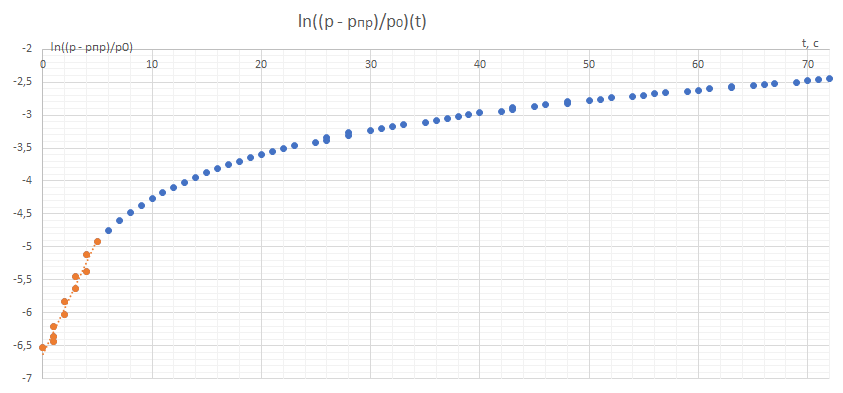
\includegraphics[width=14cm]{2.3.1_gr_1}
	\end{center}
	\label{ris8}
\end{figure}


Очевидно, что на начальном участке идет улучшение вакуума за счет насоса, утечками можно пренебречь. Тогда:

$k=\frac{<yt>-<y><t>}{<t^2>-<t>^2}$ \;\;\;\;\;\;\; $\sigma_{k}=\sqrt{\frac{1}{N}(\frac{<{y}^2>-<y>^2}{<t^2>-<t>^2}-{k}^2)}$

Т.к. число точек велико, поправка N-2 вносит небольшое значение. Вместо нее для упрощения подсчетов будем использовать N, В целях увеличения читаемости текста, логарифм по оси oY был заменен на переменную y

$k = (-0.231 \pm 0.004)c^{-1}$

$\sigma_{W}=\sqrt{(\sigma^{\text{случ}}_{W})^2+(\sigma^{\text{приб}}_{W})^2}$

Отметим, что здесь и далее, за случайные погрешности принимаются погрешности значений угловых коэффициентов графиков

$\sigma^{\text{приб}}_{W} = W\frac{\sigma{V_{\text{вв}}}}{V_{\text{вв}}}$

$W = -kV_{\text{вв}} = (0.27 \pm 0.01) \frac{\text{л}}{c}$


Рассмотрим откачивание газа. Угловой коэффициент нашего графика p(t):

Аналогично k посчитаем значение и погрешность $\alpha$

$\alpha = (0.89 \pm 0.02)*10^{-5} \frac{\text{торр}}{c}$

 Воспользуемся уравнением
\begin{equation}
V_{\text{вв}}dp = (Q_{\text{д}} + Q_{\text{и}})dt
\end{equation}
Учтем также уравнение (1) в предельном случае. Тогда аналогично W посчитаем:
\begin{equation}
Q_{\text{и}} = p_{\text{пр}}W - \alpha{V_{\text{вв}}} = (0,72 \pm 0.09)*10^{-5} \frac{\text{торр*л}}{c}
\end{equation}

$p_{\text{уст}} = 1.1*10^{-4}$ мм.рт.ст

$p_{\text{фв}} = 2,2 * 10^{-3}$ мм.рт.ст.

Запишем формулу (1) в случаях, когда капилляр открыт и закрыт и подставим в (5). Получим
\begin{equation}
W =  \frac{d^3}{6}\sqrt{\frac{2\pi{RT}}{\mu}}\frac{p_{\text{фв}}-p_{\text{уст}}}{L(p_{\text{уст}}-p_{\text{пр}})} = (0,29 \pm 0.02)\frac{\text{л}}{c}
\end{equation}

\end{enumerate}

\newpage

\section{Обсуждение результатов и выводы}

В ходе работы были достигнуты следующие цели:
\begin{itemize}
\item Получено состояние системы, приближенное к вакууму
\item Экспериментально получены и подтверждены зависимости p(t) в исследуемом диапазоне значений
\item Определены скорости откачки воздуха насосом и проникновения (утечек) воздуха извне
\end{itemize}

В ходе работы с неплохой точностью были получены значения объемов нашей системы не более 3\%, а также скорость проникновения воздуха извне (8\%) и откачки воздуха насосом (4\%). Необходимо отметить, что величины случайной погрешности дали хоть и весомый, однако не определяющий вклад, что говорит о неплохой точности проведенных измерений.

Отметим, что значения откачки воздуха насосом в двух способах измерений совпадают с хорошей точностью. Однако при втором способе измерение имеет значительную погрешность (7\%), что говорит о недостаточной точности. Объяснить это можно использование большого числа величин, требующих измерения.


\end{document}